\documentclass[letterpaper, 11pt]{article}
\usepackage{comment} % enables the use of multi-line comments (\ifx \fi) 
\usepackage{fullpage} % changes the margin
\usepackage{fancyhdr} % for footer
\usepackage[UKenglish]{isodate}% http://ctan.org/pkg/isodate for date format
\usepackage{float}%force tables/figs into certain placement
\usepackage{changepage}%for dichotomous key
\usepackage{graphicx}%for figures
\usepackage{natbib}	%for bibliography
\usepackage{subcaption}%for figures
\usepackage{hyperref}%for hyperlinks
\usepackage{multicol}% for making list span multiple columns
\usepackage[font=small,labelfont=bf]{caption}%for captions
\renewcommand{\headrulewidth}{0pt}
\newcommand*{\doi}[1]{\href{http://dx.doi.org/#1}{doi: #1}}% links DOI
\usepackage{epigrafica}%changes default font to epigrafica
\DeclareTextAccent{\"}{OT1}{168}%declare umlaut
\usepackage{placeins}%prevent images from floating into inappropriate sections
\newcommand{\latinword}[1]{\texttt{\itshape #1}}%use \latinword for vocab
\def\labelitemi{--} %change bullet to em dash
\pagestyle{fancy}

\lhead{}
\chead{}
\rhead{}
\lfoot{ENT 432 (Fall 2016) - Penn State}
\cfoot{}
\rfoot{\thepage}
\renewcommand{\footrulewidth}{0.4pt}
\title{Unit 5 - Non-hexapod Arthropoda}
\author{Open Entomology Project}
\begin{document}
\cleanlookdateon %removed ordinal date
\maketitle
\thispagestyle{fancy}
\section*{Introduction}
In this unit we learn about major non-hexapod arthropod lineages---\textbf{Chelicerata} (spiders, mites, scorpions, and their relatives), \textbf{Myriapoda} (centipedes, millipedes, and their relatives), and some non-hexapod \textbf{Pancrustacea} (pillbugs, brine shrimp, and their relatives---including our collective understanding of their natural histories and hypotheses of their evolutionary history relative to other arthropods. We'll also look at the putative sister to Arthropoda: \textbf{Onychophora} (velvet worms).

You should have a relatively firm grasp of arthropod anatomy at this point. Before we start revisit our discussion of the phenotypes that make an organism an arthropod. Now consider their diversity relative to other metazoans: vertebrates, annelids, nematodes, \textit{etc}. What phenotypes would you consider ``key innovations'' for Arthropoda? Why is Arthropoda orders of magnitude more diverse than its sister lineage?

As you examine the specimens in the hands-on portion of this unit think about how the phenotypes you observe inform us of the evolutionary history of these organisms.

\section*{Materials}
\begin{itemize}
\item specimens (provided)
\item fine forceps, probes (provided)
\item sorting tray, watch glasses, gloves, safety glasses, glycerol, ethanol (provided)
\item pencil/lab notebook for sketches
\end{itemize}

\section*{Safety}
We will be working with sharp tools. Wear your personal protective gear at all times. Specimens are to be returned to their vials after lab, and glycerine and ethanol will be collected for proper disposal or reuse.

\section*{Methods}
Working with a partner, organize your space, specimens, tools, and microscope. Use your probe and forceps to manipulate the specimen. In this lab, however, we will not be dissecting specimens (unless otherwise noted). You can start anywhere in the handout.

\section{Onychophora (velvet worms)}
\noindent{}\textit{Diagnostic characters:} Segmented and relatively soft-bodied, with a single pair of antennae and serially homologous legs. Spiracles and tracheae present.\\

\noindent{}\textit{Natural history:} Velvet worms are predators of other invertebrates, usually subduing prey with a glue-like mucous that is excreted with force from glands near the mouth. They are quite susceptible to desiccation and so are usually found in humid habitats. There are approximately 200 species, which can found throughout the Neotropics and in pockets throughout the rest of the world. There is a rich fossil record from marine environments, but there are no extant marine species.\\

\hangindent2em\textbf{Question 5-1:} Can you see any shared, derived characters (Figure \ref{fig:onych}) between onychophorans and arthropods? What features indicate that these creatures are definitely \textit{not} Arthropoda (\textit{i.e.}, how would you write the diagnosis)? 

\begin{figure}[ht!]
  \centering
    \includegraphics[width=0.9\textwidth]{onych}
  \caption{Photo (CC BY-NC-SA 2.0) by Yonatan Monk: \url{https://flic.kr/p/85z27d}}.
  \label{fig:onych}
\end{figure}

\section{Chelicerata}
These arthropods generally share the following characters: 
\begin{itemize}
\item antennae absent (though anteriormost pair of legs often antenniform)
\item 6 pairs of uniramous appendages: chelicerae (mouthparts) + pedipalps + 4 pairs of legs
\item 2 tagmata: prosoma (cephalothorax) and opisthosoma (abdomen)
\end{itemize}
The most diverse group of chelicerates is Arachnida, which includes all the terrestrial species of Chelicerata. We will examine specimens of the taxa listed below. Can you see the diagnostic characters clearly? If you saw any of these specimens in a lab practical could you name it (with correct spelling), describe a diagnostic feature, and/or describe its natural history?

\subsection{Araneae (spiders)}
\noindent{}\textit{Diagnostic characters:} Chelicerae fang-like (Figure \ref{fig:fang}); anteriormost pair of legs not antenniform; pedipalps not chelate (\textit{i.e.}, pincer/claw-shaped), rarely stouter than legs; opisthosoma not obviously segmented (except rarely); opisthosoma attached to prosoma via narrow constriction (Figure \ref{fig:spider}); spinnerets present posteroventrally on opisthosoma, but no tail-like structure (telson).\\

\noindent{}\textit{Natural History:} Incredibly diverse taxon, with more than 45,000 described species found worldwide and in almost every habitat. These arthropods are well known for their use of silk to form webs, tunnels, ``parachutes'', and other contraptions.\\

\hangindent2em\textbf{Question 5-2:} Why do spiders have a constricted ``waist''? What are fang-like chelicerae adapted for? Can you predict how they're used?

\begin{figure}[ht!]
    \centering
    \begin{subfigure}[ht!]{0.25\textwidth}
        \includegraphics[width=\textwidth]{fang}
        \caption{Chelicerae. Photo (CC BY-SA 2.0) by Matt Reinbold: \url{https://flic.kr/p/2Bxryh}}
        \label{fig:fang}
    \end{subfigure}
    ~ %add desired spacing between images, e. g. ~, \quad, \qquad, \hfill etc. 
      %(or a blank line to force the subfigure onto a new line)
    \begin{subfigure}[ht!]{0.65\textwidth}
        \includegraphics[width=\textwidth]{spider}
        \caption{Ventral habitus. Photo (CC BY-SA 2.0) by James E. Petts: \url{https://flic.kr/p/fJqUsE}}
        \label{fig:spider}
    \end{subfigure}
    \caption{Spiders (Araneae)}\label{fig:spiders}
\end{figure}

\subsection{Acari (mites, ticks)}
\noindent{}\textit{Diagnostic characters:} Opisthosoma not segmented (See Figure \ref{fig:mites}); opisthosoma broadly joined to prosoma, no tail-like structure (telson); young instars with 3 pairs of legs, adults with 4; pedipalps not chelate, not thicker than legs; mouthparts usually project anteriorly, chelicerae not chelate; usually very small (0.08--10 mm body length).\\

\noindent{}\textit{Natural History:} Another incredibly diverse taxon, with more than 48,000 described species found worldwide. It is difficult to generalize their natural history, as there are species that feed as predators, herbivores, detritivores, fungivores, and parasites, and they live in just about every habitat imaginable.  \\

\hangindent2em\textbf{Question 5-3:} Based on their mouthpart morphology can you make \textit{any} generalization or predictions about their feeding habits?\\

\begin{figure}[ht!]
    \centering
    \begin{subfigure}[ht!]{0.5\textwidth}
        \includegraphics[width=\textwidth]{mite1}
        \caption{Dorsal habitus. Photo (CC BY 2.0) by Mick E. Talbot: \url{https://flic.kr/p/55WxVw}}
        \label{fig:mite1}
    \end{subfigure}
    ~ %add desired spacing between images, e. g. ~, \quad, \qquad, \hfill etc. 
      %(or a blank line to force the subfigure onto a new line)
    \begin{subfigure}[ht!]{0.4\textwidth}
        \includegraphics[width=\textwidth]{mite2}
        \caption{Dorsal habitus. Photo (CC BY 2.0) by Mick E. Talbot: \url{https://flic.kr/p/6s36QX}}
        \label{fig:mite2}
    \end{subfigure}
    \caption{Mites (Acari).} \label{fig:mites}
\end{figure}

\subsection{Opiliones (harvestmen, daddy-longlegs)}
\noindent{}\textit{Diagnostic characters:} Chelicerae chelate; opisthosoma segmented, broadly joined to prosoma, without tail-like structure (telson) (Figures \ref{fig:opiliones1}--\ref{fig:opiliones2}); body ovoid; body  \textless7 mm long usually, with leg span up to 160 mm; pedipalp morphology variable: usually thinner than legs, sometimes raptorial.\\

\noindent{}\textit{Natural history:} Most species are predators and/or scavengers, feeding with a compound structure (stomotheca), formed, in part, by the proximal pedipalp and anteriormost leg segments. These arachnids lack venom and silk glands but do produce noxious defensive odors through scent gland openings (ozopores). There are more than 6,500 species worldwide. \\

\begin{figure}[ht!]
  \centering
    \includegraphics[width=0.7\textwidth]{opiliones1}
  \caption{Opiliones. Photo (CC BY-SA 2.0) by Gordon: \url{https://flic.kr/p/bVW3Yp}}
  \label{fig:opiliones1}
\end{figure}

\begin{figure}[ht!]
  \centering
    \includegraphics[width=0.7\textwidth]{opiliones2}
  \caption{Opiliones. Photo (CC BY 2.0) by Thomas Bresson: \url{https://flic.kr/p/6ytEzH}}
  \label{fig:opiliones2}
\end{figure}
\hangindent2em\textbf{Question 5-4:} Like all arachnids, Opiliones do not have antennae. Can you find an appendage that serves a similar function? Given the variation in pedipalp morphology across Opiliones, what would you predict is the function of these appendages?

\FloatBarrier
\subsection{Scorpiones (scorpions)}
\noindent{}\textit{Diagnostic characters:} Chelicerae chelate; pedipalps long, chelate, and usually at least as thick as legs (Figure \ref{fig:scorpion}); anteriormost pair of legs used for walking (\textit{i.e.}, not antenniform); opisthosoma segmented, broadly joined to prosoma; tail-like posteriorly (tail = telson); telson with venom gland and sting present; 2nd segment of opisthosoma with comblike organs (pectines) ventrally.\\

\noindent{}\textit{Natural history:} There are more than 1,700 species found worldwide, all of which are predators.\\

\begin{figure}[ht!]
  \centering
    \includegraphics[width=0.7\textwidth]{scorpion}
  \caption{Scorpiones. Photo (CC BY 2.0) by Clinton \& Charles Robertson: \url{https://flic.kr/p/t52BX}}
  \label{fig:scorpion}
\end{figure}
\hangindent2em\textbf{Question 5-5:} Some scorpion species have massive pedipalps and relatively small telsons, while others exhibit the opposite set of phenotypes (\textit{i.e.}, massive telsons but small pedipalps); from a natural history perspective what do you think is happening with these structures? Also, how do you think scorpions find prey?\vspace{5cm}

\subsection{Pseudoscorpiones (pseudoscorpions)}
\noindent{}\textit{Diagnostic characters:} Chelicerae chelate; pedipalps long, chelate, and thicker than legs (Figure \ref{fig:pseudo}); anteriormost pair of legs used for walking (\textit{i.e.}, not antenniform); opisthosoma segmented, broadly joined to prosoma, without telson; patellar segment absent on legs.\\

\noindent{}\textit{Natural history:} There are 3,300 species of pseudoscorpion, most of which are relatively small (\textless5 mm long). Sometimes they can be found clinging to insects, hitching a ride (phoresy) or possibly eating parasitic mites. Some species subdue prey with venom, from a gland in the pedipalp.\\

\begin{figure}[ht!]
  \centering
    \includegraphics[width=0.7\textwidth]{pseudo}
  \caption{Pseudoscorpionida. Photo (CC BY-SA 2.0) by Gilles San Martin: \url{https://flic.kr/p/5Nxymf}}
  \label{fig:pseudo}
\end{figure}

\section{Myriapoda}
\begin{itemize}
\item antennae present as single pair
\item appendages uniramous (\textit{i.e.}, no branches)
\item mouthparts mandibulate (\textit{i.e.}, not chelicerate)
\end{itemize}

\subsection{Diplopoda (millipedes)}
\noindent{}\textit{Diagnostic characters:} Most (apparent) segments with 2 pairs of legs (Figure \ref{fig:diplop2}); antennae usually 7-segmented, short; 30+ pairs of legs present usually; body usually round, tube-like; some species small, bristly (Figure \ref{fig:diplop1}).\\

\noindent{}\textit{Natural history:} Millipedes typically forage on rotting materials (saprophagy) and are important recyclers of nutritive material. Most species are harmless, although some are renown for excreting toxic compounds when handled. There are \textgreater12,000 species described worldwide.\\

\begin{figure}[ht!]
    \centering
    \begin{subfigure}[ht!]{0.35\textwidth}
        \includegraphics[width=\textwidth]{diplop1}
        \caption{Photo (CC BY 2.0) by Gilles San Martin: \url{https://flic.kr/p/dgF295}}
        \label{fig:diplop1}
    \end{subfigure}
    ~ %add desired spacing between images, e. g. ~, \quad, \qquad, \hfill etc. 
      %(or a blank line to force the subfigure onto a new line)
    \begin{subfigure}[ht!]{0.55\textwidth}
        \includegraphics[width=\textwidth]{diplop2}
        \caption{Photo (CC BY 2.0) by Brian Gratwicke: \url{https://flic.kr/p/dFP5Wu}}
        \label{fig:diplop2}
    \end{subfigure}
    \caption{Millipedes (Diplopoda).} \label{fig:diplopoda}
\end{figure}

\subsection{Chilopoda (centipedes)}
\noindent{}\textit{Diagnostic characters:} Antennae usually with 14+ segments; apices of anteriormost pair of legs (forcipules) modified into fang-like structures (Figure \ref{fig:chilo2}); most segments with 1 pair of legs; 15+ pairs of legs present usually (Figures \ref{fig:chilo1}--\ref{fig:chilo2}); body usually dorsoventrally flattened (but see Figure \ref{fig:chilo1}).\\

\noindent{}\textit{Natural history:} \\

\begin{figure}[ht!]
    \centering
        \includegraphics[width=0.7\textwidth]{chilo1}
        \caption{Chilopoda. Photo (CC BY 2.0) by Brian Gratwicke: \url{https://flic.kr/p/ehk44m}}
        \label{fig:chilo1}
\end{figure}

\begin{figure}[ht!]
	\centering
        \includegraphics[width=0.7\textwidth]{chilo2}
        \caption{Chilopoda. Photo (CC BY 2.0) by Derrick Coetzee: \url{https://flic.kr/p/cF2Czu}}
        \label{fig:chilo2}
\end{figure}

\noindent{}Based on your observations of the two myriapod taxa we have in lab, what would you say about their natural history? Where does each taxon typically live, and what does it eat?\vspace{4cm}

\section{Non-hexapod Pancrustacea (formerly ``Crustacea'')}
\begin{itemize}
\item often with 2 tagmata: cephalothorax and abdomen
\item many biramous (2-branched) appendages, usually with 2nd pair of antennae (antennules)
\item mouthparts mandibulate
\end{itemize}

\subsection{Isopoda (pillbugs, sowbugs)}
\noindent{}\textit{Diagnostic characters:} Body with no carapace, usually dorso-ventrally flattened (Figures \ref{fig:isopod1}--\ref{fig:isopod2}); 7 pairs of thoracic legs; 2nd pair of antennae reduced.\\

\noindent{}\textit{Natural history:} One of the few non-hexapod pancrustaceans to radiate in the terrestrial environment. Of the approximately 10,000 known species, about half are terrestrial. The rest are marine (about 4,500 spp.) or inhabit freshwater. Most species survive as scavengers but many are parasitic on fish or other aquatic organisms.\\

\begin{figure}[ht!]
    \centering
    \begin{subfigure}[ht!]{0.55\textwidth}
        \includegraphics[width=\textwidth]{isopod}
        \caption{Photo (CC BY 2.0) by Mick Talbot \url{https://flic.kr/p/6vEqLt}}
        \label{fig:isopod1}
    \end{subfigure}
    ~ %add desired spacing between images, e. g. ~, \quad, \qquad, \hfill etc. 
      %(or a blank line to force the subfigure onto a new line)
    \begin{subfigure}[ht!]{0.35\textwidth}
        \includegraphics[width=\textwidth]{isopod2}
        \caption{Photo (CC BY 2.0) by Mick Talbot \url{https://flic.kr/p/6jQM1g}}
        \label{fig:isopod2}
    \end{subfigure}
    \caption{Isopoda} \label{fig:isopoda}
\end{figure}

\subsection{Amphipoda (scuds)}
\noindent{}\textit{Diagnostic characters:} No carapace, usually laterally flattened (Figure \ref{fig:amphip}); fore legs often raptorial; usually 6 or 7 pairs of thoracic legs.\\

\noindent{}\textit{Natural history:} Of the 9,500 known species, approximately 20\% are found in freshwater. The vast majority are marine, but a handful are terrestrial (usually closely associated with aquatic habitats). They are mostly scavengers.\\

\begin{figure}[ht!]
  \centering
    \includegraphics[width=0.65\textwidth]{amphip}
  \caption{Amphipoda. Photo (CC BY-NC 2.0) by Fred Snyder:  \url{https://flic.kr/p/9vTru1}}
  \label{fig:amphip}
\end{figure}

\noindent{}Given your observations of these ``crustaceans'', why do we have so few terrestrial and fresh water species, relative to insects? \\

\subsection{Test your skills!}
You've now seen a handful of arthropod taxa, from three groups that are not insects. While they are not the focus of this course, these organisms are incredibly diverse and remain relevant to understanding the evolution of Arthropoda. Take some time to observe specimens of taxa we are not covering, bask in the diversity of phenotypes, and see if you can classify them correctly. Are the chelicerates, myriapods, or pancrustaceans? Why or why not? Draw and/or describe features you think are diagnostic. Based on their morphology, can you predict their natural history?

\subsubsection*{Solifugae (Solpugida; camelspiders, sunspiders, windscorpions)}
What group does it belong in and why?\\

\noindent{}What diagnostic characters separate it from the taxa above?\\

\noindent{}What do these arthropods eat, and how do they live?\\

\begin{figure}[ht!]
  \centering
    \includegraphics[width=0.6\textwidth]{solfugida}
  \caption{Solifugae. Photo (CC BY 2.0) by Maximilian Paradiz: \url{https://flic.kr/p/7J7B3r}}
  \label{fig:solfugida}
\end{figure}

\subsubsection*{Decapoda (crabs, lobsters, shrimp)}
What group does it belong in and why?\\

\noindent{}What diagnostic characters separate it from the taxa above?\\

\noindent{}What do these arthropods eat, and how do they live?\\

\begin{figure}[ht!]
  \centering
    \includegraphics[width=0.6\textwidth]{decapod}
  \caption{Decapoda. Photo (CC BY 2.0) by Guenter Schuster: \url{https://flic.kr/p/njkdZ3}}.
  \label{fig:decapoda}
\end{figure}

\subsubsection*{Thelyphonida (Uropygi, Uropygida, vinegaroons, whipscorpions)}
What group does it belong in and why?\\

\noindent{}What diagnostic characters separate it from the taxa above?\\

\noindent{}What do these arthropods eat, and how do they live?\\

\begin{figure}[ht!]
  \centering
    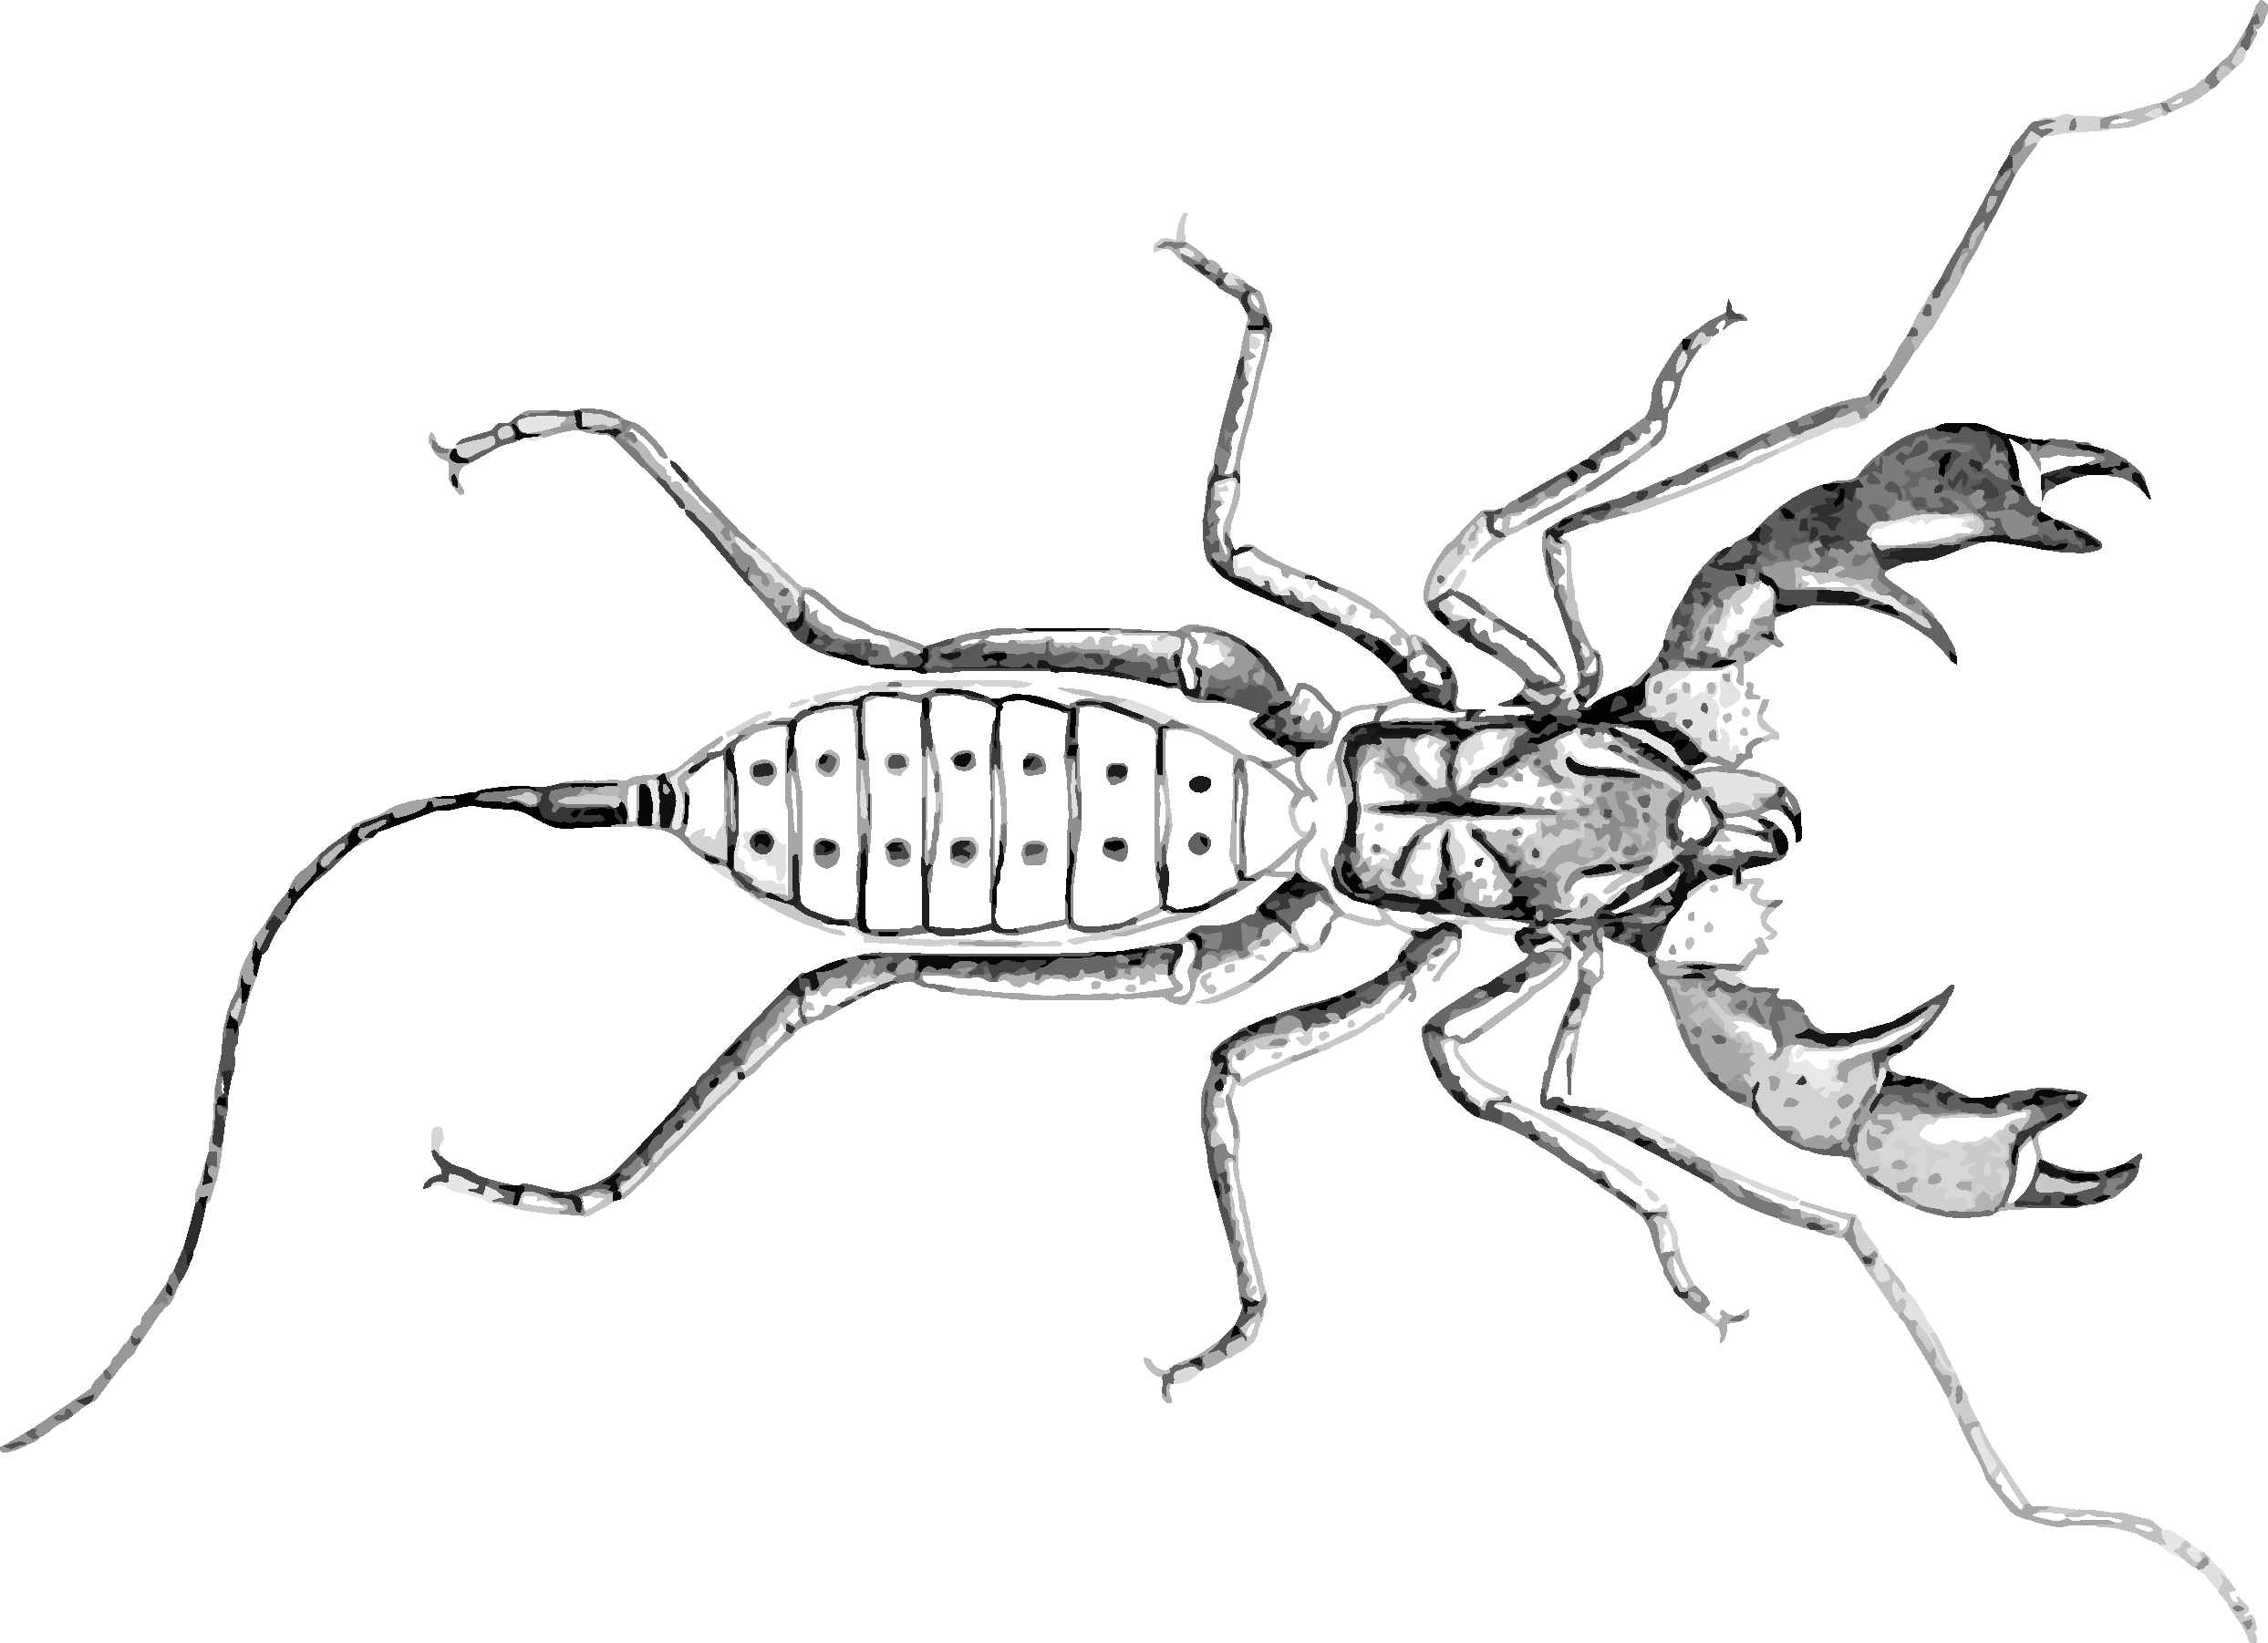
\includegraphics[width=0.6\textwidth]{thelyphonida}
  \caption{Thelyphonida. Photo (CC BY-NC-SA 2.0) by StarWatcher307: \url{https://flic.kr/p/8hde2g}}
  \label{fig:thelyphonida}
\end{figure}

\subsubsection*{Amblypygi (tail-less whipscorpions)}
What group does it belong in and why?\\

\noindent{}What diagnostic characters separate it from the taxa above?\\

\noindent{}What do these arthropods eat, and how do they live?\\

\begin{figure}[ht!]
  \centering
    \includegraphics[width=0.6\textwidth]{ambly1}
  \caption{Amblypygi. Photo (CC BY-NC-SA 2.0) by Jos\'{e} Eugenio G\'{o}mez Rodr\'{i}guez: \url{https://flic.kr/p/5hmWNS} }
  \label{fig:ambly1}
\end{figure}

\subsubsection*{Xiphosura (horseshoe crabs)}
What group does it belong in and why?\\

\noindent{}What diagnostic characters separate it from the taxa above?\\

\noindent{}What do these arthropods eat, and how do they live?\\

\begin{figure}[ht!]
  \centering
    \includegraphics[width=0.6\textwidth]{xipho}
  \caption{Xiphosura. Photo (CC BY-ND 2.0) NH Sea Grant: https://flic.kr/p/duEyis: \url{https://flic.kr/p/85z27d}}.
  \label{fig:xipho}
\end{figure}

\subsubsection*{Copepoda (copepods, fish lice)}
What group does it belong in and why?\\

\noindent{}What diagnostic characters separate it from the taxa above?\\

\noindent{}What do these arthropods eat, and how do they live?\\

\begin{figure}[ht!]
  \centering
    \includegraphics[width=0.6\textwidth]{copepod}
  \caption{Copepod from Ten Acre Pond (Centre Co., Pennsylvania). Photo (CC BY 2.0) by Andy Deans: \url{https://flic.kr/p/nsJuJZ}}
  \label{fig:copepod}
\end{figure}

\subsubsection*{Symphyla (symphylans)}
What group does it belong in and why?\\

\noindent{}What diagnostic characters separate it from the taxa above?\\

\noindent{}What do these arthropods eat, and how do they live?\\

\begin{figure}[ht!]
  \centering
    \includegraphics[width=0.6\textwidth]{Symphyla}
  \caption{Symphyla. Photo (CC BY-SA 3.0) by Sonia Martinez: \url{http://bit.ly/1iRxA29}}
  \label{fig:symphyla}
\end{figure}

\noindent{}Can you draw a phylogeny showing the relationships between Onychophora, Chelicerata, Myriapoda, and Pancrustacea (including Hexapoda)? Which node is the common ancestor of Arthropoda? \citep[Hint: see][]{Dunlop2013}\\

\section*{Epilogue}
This handout is part of an open curriculum. Original files are available free for anyone to download, copy, modify, and improve at the Open Entomology GitHub repository \citep{ENT432}, which also provides a mechanism for reporting problems and other feedback:\\
\url{https://github.com/OpenEntomology/InsectBiodiversityEvolution/issues}

\section*{Acknowledgments}
Images were borrowed from Wikimedia Commons, Flickr, and the Biodiversity Heritage Library. The authors made a good faith effort to adhere to the terms of their respective Creative Commons licenses and provide appropriate credit and links to source pages. All images were accessed 19 August 2016. We thank these artists for making their images available for educational purposes.


\FloatBarrier
% adding bibliography here
\bibliographystyle{myplainnat}
\bibliography{bib}

\end{document}

